\documentclass[12pt]{article}
\usepackage[spanish]{babel}
\usepackage[utf8]{inputenc}
\usepackage{amsmath}
\usepackage{graphicx}
\usepackage{booktabs}
\usepackage{array}
\usepackage{multirow}
\usepackage{float}
\usepackage{longtable}
\usepackage{subcaption}
\usepackage{wrapfig}
\usepackage{tikz}
\usetikzlibrary{arrows.meta, positioning, shapes.geometric}
\title{Proyecto 3: Reemplazo de Equipos}
\author{Emily Sanchez \\ Viviana Vargas \\[1cm] Curso: Investigación de Operaciones \\ II Semestre 2025}
\date{\today}

\begin{document}

\maketitle
\newpage
\section*{Problema de Reemplazo de Equipos}
El problema consiste en determinar el momento óptimo para reemplazar un equipo durante un período de planificación.\\
\textbf{Fórmula del costo:} $C_{t,j} = \text{Compra} + \sum_{k=1}^{j-t} \text{Mantenimiento}_k - \text{Venta}_{j-t}$\\
\textbf{Algoritmo:} Programación Dinámica hacia atrás\\
\textbf{Función recursiva:} $g(t) = \min\limits_{j=t+1}^{\min(t+\text{vida útil}, n)} \{C_{t,j} + g(j)\}$ con $g(n) = 0$\\

\section*{Datos del Problema}
\begin{itemize}
\item Costo inicial (compra): \$500,00
\item Plazo del proyecto: 5 años
\item Vida útil del equipo: 3 años
\end{itemize}

\begin{table}[H]
\centering
\caption{Datos del equipo por año de uso}
\begin{tabular}{ccc}
\toprule
Año de Uso & Mantenimiento & Valor Residual \\
\midrule
1 & \$400,00 & \$30,00 \\
2 & \$300,00 & \$40,00 \\
3 & \$250,00 & \$60,00 \\
\bottomrule
\end{tabular}
\end{table}

\clearpage
\section*{Cálculo de Costos $C_{t,j}$}
\begin{longtable}{cccc}
\caption{Cálculo detallado de costos por período} \\
\toprule
Período (t-j) & Duración & Fórmula & Costo \\
\midrule
\endfirsthead
\multicolumn{4}{c}{\tablename\ \thetable\ -- Continúa} \\
\toprule
Período (t-j) & Duración & Fórmula & Costo \\
\midrule
\endhead
\midrule
\multicolumn{4}{r}{Continúa en la siguiente página} \\
\endfoot
\bottomrule
\endlastfoot
0-1 & 1 año & $500 + 400 - 30$ & \$870,00 \\
0-2 & 2 años & $500 + 400 + 300 - 40$ & \$1160,00 \\
0-3 & 3 años & $500 + 400 + 300 + 250 - 60$ & \$1390,00 \\
1-2 & 1 año & $500 + 400 - 30$ & \$870,00 \\
1-3 & 2 años & $500 + 400 + 300 - 40$ & \$1160,00 \\
1-4 & 3 años & $500 + 400 + 300 + 250 - 60$ & \$1390,00 \\
2-3 & 1 año & $500 + 400 - 30$ & \$870,00 \\
2-4 & 2 años & $500 + 400 + 300 - 40$ & \$1160,00 \\
2-5 & 3 años & $500 + 400 + 300 + 250 - 60$ & \$1390,00 \\
3-4 & 1 año & $500 + 400 - 30$ & \$870,00 \\
3-5 & 2 años & $500 + 400 + 300 - 40$ & \$1160,00 \\
4-5 & 1 año & $500 + 400 - 30$ & \$870,00 \\
\end{longtable}

\clearpage
\section*{Cálculo de $g(t)$ (Programación Dinámica)}
\begin{itemize}
\item $g(5) = 0$ (caso base)
\item $g(4) = \min\{ C_{4,5} + g(5) = 870,00\} = \$870,00$
\item $g(3) = \min\{ C_{3,4} + g(4) = 1740,00, C_{3,5} + g(5) = 1160,00\} = \$1160,00$
\item $g(2) = \min\{ C_{2,3} + g(3) = 2030,00, C_{2,4} + g(4) = 2030,00, C_{2,5} + g(5) = 1390,00\} = \$1390,00$
\item $g(1) = \min\{ C_{1,2} + g(2) = 2260,00, C_{1,3} + g(3) = 2320,00, C_{1,4} + g(4) = 2260,00\} = \$2260,00$
\item $g(0) = \min\{ C_{0,1} + g(1) = 3130,00, C_{0,2} + g(2) = 2550,00, C_{0,3} + g(3) = 2550,00\} = \$2550,00$
\end{itemize}

\clearpage
\section*{Solución Óptima}
\textbf{Costo mínimo total:} \$2550,00\\
\textbf{Planes óptimos encontrados:} 2
\subsection*{Grafos de Planes Óptimos}
A continuación se presentan los grafos de \emph{saltos de rana} para cada plan óptimo encontrado.

\begin{figure}[H]
\centering
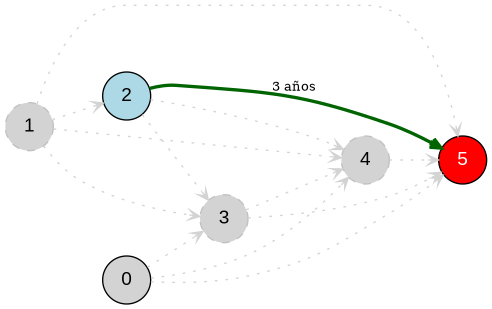
\includegraphics[width=0.9\textwidth]{Remplazo1111_plan_1.png}
\caption{Plan Óptimo 1: \texttt{0-2-5} (Todos los períodos mostrados)}
\textbf{Leyenda:} \textcolor{green}{\bullet} Inicio, \textcolor{red}{\bullet} Fin, \textcolor{blue}{\bullet} Usado, \textcolor{gray}{\bullet} No usado, \textcolor{darkgreen}{\rightarrow} Salto óptimo, \textcolor{gray}{\dashrightarrow} Salto potencial
\label{fig:plan1}
\end{figure}

\textbf{Plan 1:} \texttt{0-2-5}
\begin{itemize}\small
\item Período 0-2: 2 años, Costo: \$1160,00
\item Período 2-5: 3 años, Costo: \$1390,00
\end{itemize}

\begin{figure}[H]
\centering
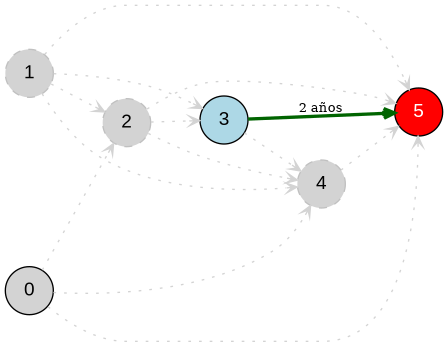
\includegraphics[width=0.9\textwidth]{Remplazo1111_plan_2.png}
\caption{Plan Óptimo 2: \texttt{0-3-5} (Todos los períodos mostrados)}
\textbf{Leyenda:} \textcolor{green}{\bullet} Inicio, \textcolor{red}{\bullet} Fin, \textcolor{blue}{\bullet} Usado, \textcolor{gray}{\bullet} No usado, \textcolor{darkgreen}{\rightarrow} Salto óptimo, \textcolor{gray}{\dashrightarrow} Salto potencial
\label{fig:plan2}
\end{figure}

\textbf{Plan 2:} \texttt{0-3-5}
\begin{itemize}\small
\item Período 0-3: 3 años, Costo: \$1390,00
\item Período 3-5: 2 años, Costo: \$1160,00
\end{itemize}

\end{document}
